\section{RESULTS}\label{sec3}%Results
%% topic 1 spectral measures (behavioral relevance and physiological distribution on free ears)
%figure box A - F: Free Ears: VSI across bands, VSI LR and VSI RMSE 
\begin{wrapfigure}[31]{r}{9.5cm}
\captionsetup{width=9cm}
\centering
    \raisebox{0pt}[\dimexpr\height-1.4\baselineskip\relax]{
        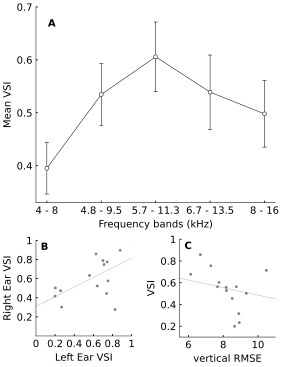
\includegraphics[width=9cm]{../Results/figures/fig2/fig2}}
	\caption{Free ears VSI and localization performance. \textbf{A}, Variation of VSI across five octave bands between 4 and 16kHz. VSI was averaged across sets of DTFs obtained from participants' left and right ears without earmolds. VSI varies significantly and is highest in the 5.7–11.3 kHz band.  \textbf{B}, Left and right ear VSI of each participant in the 5.7-11.3 kHz band. VSIs of the left and right ears were similar. \textbf{C}, Relation between VSI in the 5.7 – 13.5 kHz band and vertical localization accuracy.}
	\label{fig:ef_vsi}
\end{wrapfigure}
\noindent\vspace{-3\baselineskip}

\subsection{VSI and localization performance with free ears were related}

Participants' directional transfer functions (DTFs) were recorded across the vertical midline with and without earmolds. To quantify spectral information available for vertical sound localization in the individual sets of DTFs, VSI \citep{trapeau_fast_2016} and spectral strength \citep{andeol_sound_2013} were computed in 5 octave bands between 4 and 16 kHz (4–8 kHz, 4.8–9.5 kHz, 5.7–11.3 kHz, 6.7–13.5kHz, 8–16kHz). Spectral information of participants’ free ears varied among frequency bands (Kruskal-Wallis test, VSI: $p = 0.0087$, spectral strength: $p = 10^{-7}$). The dissimilarity between DTFs across elevations (VSI) peaked in the 5.7–11.3 kHz band as previously reported by \citet{trapeau_fast_2016} (\cref{fig:ef_vsi} A). The VSIs of all participants in this band are shown in \cref{fig:ef_vsi} B. Participants' left and right ears had similar VSI (Spearman correlation between the VSI of left and right ears in the 5.7–11.3 kHz band: $r = 0.45, p = 0.0897$). Spectral strength, i.e., the variance within individual DTFs, indicated the highest spectral detail in the neighboring 6.7–13.5 kHz band. When joining these two bands for the analysis, VSI correlated with vertical localization accuracy (\cref{fig:ef_vsi} C) and vertical SD (free ears VSI in the 5.7–13.5 kHz band compared to vertical localization: RMSE: R = -0.58, $p = 0.0249$, EG: R = 0.15, $p = 0.6025$, SD: R = -0.58, $p = 0.0249$). No correlation was found between behavioral metrics and VSI in the other frequency bands. Spectral strength did not correlate with behavior in the tested frequency bands.

%% topic 2 spectral effect of molds (spectral impact of molds, physiological plausibility, distribution across participants, m1m2 spectral compare)
\subsection{Earmolds reduced spectral information in the 5.7–11.3 kHz band}

Application of silicone molds to the Pinnae altered spectral cues in the 4–16 kHz band. The consecutively applied sets of earmolds (further denoted as molds 1 and molds 2) attenuated the spectral notch situated in the 5–11 kHz band and the neighbouring spectral peak in the 11–14 kHz band (\cref{fig:spectral_change}, A-C). Similar effects have been observed in previous studies using pinna modifications to alter spectral cues for sound localization (\citet{trapeau_fast_2016}, \citet{wanrooij_relearning_2005}, \citet{hofman_relearning_1998}). Comparing VSIs of participants' modified and free ears in the 5.7–11.3 kHz band showed that earmolds reduced the amount of spectral information available for elevation discrimination in this band (\cref{fig:molds_vsi} B, differences between VSI of free and modified ears; free ears: 0.61 $\pm$ 0.04, vs molds 1: 0.45 $\pm$ 0.05, $p = 0.0022$, vs molds 2: 0.39 $\pm$ 0.04, $p = 0.0036$). The two sets of earmolds led to similar levels of VSI reduction compared to participants' free ears (free ears VSI reduction caused by molds 1: 0.18 $\pm$ 0.06 vs molds 2: 0.18 $\pm$ 0.06, $p = 0.1973$).The relation between VSIs of participants' left and right ears persisted after mold insertion but was not significant for the second pair of earmolds (molds 1: $r = 0.56, p = 0.0336$, molds 2: $r = 0.53, p = 0.064$). \cref{fig:molds_vsi} A shows the VSI of all participants with modified and free ears. \citet{wanrooij_relearning_2005} reported the formation of new acoustic cues at higher frequencies after the insertion of silicone molds. To test whether volume reduction of pinna cavities caused by the silicone molds increased the frequencies of spectral features, spectral information was additionally compared in the 11.3–13.5 kHz band. The first set of earmolds increased VSI in this band compared to free ears (differences between VSI of free and modified ears in the 11.3–13.5 kHz band; free ears: 0.5 $\pm$ 0.06, vs molds 1: 0.64 $\pm$ 0.07, $p = 0.0387$).


\subsection{Acoustic changes occurred at similar frequencies across participants and were different between consecutive molds}

%Acoustic changes induced by the first and second set at different frequencies..  Frequencies affected by each set of earmolds were different between the first and second mold and similar across participants for each set..
 
To confirm whether spectral changes were induced at similar frequencies across participants for each set of earmolds but at different frequencies between the two sets, the probability of spectral change caused by pinna modifications was mapped for each frequency bin and elevation (\cref{fig:spectral_change} D-F). Spectral changes were defined as the absolute differences between DTFs measured before and after mold insertion above a given threshold. This threshold was a participant-specific measure of spectral difference across DTFs with free ears and was defined by the mean RMS difference across all combinations of DTFs (in dB) at each elevation (average across participants: 4.89 dB $\pm$ 0.15). Based on these thresholds, binary maps of spectral changes were created for each set of molds and participant (above-threshold changes were set to 1, all other values were set to 0). The average of these maps across participants shows the proportion of participants for which earmolds induced spectral changes above the threshold at each frequency bin and elevation.

%figure box A - F: DTFs of free vs modified ears and spectral change p
\begin{figure}[h]
\centering
	\centerline{\includegraphics[width=15cm, center]{../Results/figures/fig3/fig3}}
	\caption{Acoustic effect of the earmolds. \textbf{A}, Mean across participants' DTFs with free ears. \textbf{B-C}, Mean across participants' DTFs with modified ears. Earmolds attenuated spectral notches and peaks in the 5-14 kHz frequency range. \textbf{D-E}, Probability maps showing the proportion of participants for which the molds induced marked changes in spectral amplitude at each elevation and frequency bin. Acoustic changes induced by each set of molds occurred at similar frequencies across participants. \textbf{F}, Probability map showing the proportion of marked changes between the first and second pair of earmolds. Both sets induced acoustic changes at different frequencies.}
        \label{fig:spectral_change}
\end{figure}

% Figure box VSI and VSI dissimilarities across conditions
\begin{figure}[t]
\floatbox[{\capbeside\thisfloatsetup{capbesideposition={right,top},capbesidewidth=8cm}}]{figure}[\FBwidth]
{\caption{VSI and VSI dissimilarity across pinna shapes. \textbf{A}, Left and right ear VSI in the 5.7–11.3 kHz band. Each dot represents one participant. Grey dots show VSI values of free ears, blue and red dots represent VSI values with earmolds 1 and 2, respectively. Relations between left and right ear VSI are shown by regression lines. The similarity between left and right ear VSI persisted after mold insertion. \textbf{B}, VSI with and without molds in the 5.7–11.3 kHz band. Both sets of molds reduced VSI significantly. \textbf{C}, VSI dissimilarities across participants in the 5.7-13.5 kHz band. Grey dots show the VSI dissimilarity of free left and right ears between all combinations of two participants. Each colored dot shows the VSI dissimilarity between pinna shapes of one participant. Blue and red dots indicate dissimilarity between free ears and the first and second set of molds, respectively. Yellow dots indicate VSI dissimilarity between both sets of earmolds. The outline of the grey dot cloud largely includes the colored dots, indicating that acoustic differences induced by the molds did not exceed acoustic differences between participants' natural ears. \textbf{D}, VSI dissimilarities between the three pinna shapes in the 5.7-13.5 kHz band. VSI dissimilarity between free ears and the first earmolds was similar to VSI dissimilarity between the first and second set of molds.}
\label{fig:molds_vsi}}
{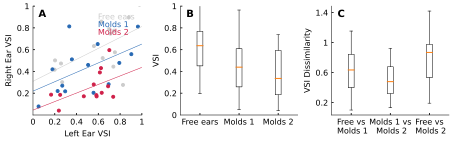
\includegraphics[width=10cm]{../Results/figures/fig4/fig4}}
\end{figure}

\subsection{Consecutive pinna modifications were equally dissimilar and physiologically plausible}

Each pair of earmolds modified the previously adapted set of DTFs. To test whether spectral differences that were consecutively induced by the molds were in the same range, VSI dissimilarities between the three different pinna shapes (ears free, earmolds 1 and earmolds 2) were computed in the 5.7–13.5 kHz frequency band. The dissimilarity between participants' free ears and the first set of earmolds was comparable to the dissimilarity between the first and the second set of molds (\cref{fig:molds_vsi} D, VSI dissimilarity in the 5.7–13.5 kHz band, free ears and molds 1:  0.64 $\pm$ 0.06 vs molds 1 and molds 2:  0.51 $\pm$ 0.05: $p = 0.2544$). The second set of earmolds induced larger spectral differences to participants' free ears than the first set (VSI dissimilarity free ears and molds 1:  0.64 $\pm$ 0.06 vs free ears and molds 2: 0.8 $\pm$ 0.06; $p = 0.0005$). To confirm that spectral changes induced by the earmolds were physiologically plausible, VSI dissimilarities between free and modified ears of each participant were compared to VSI dissimilarities between all possible pairs of participants’ free ears (\cref{fig:molds_vsi} C). The overlap of distributions shows that spectral changes induced by both sets of molds were comparable in magnitude to the natural spectrum of differences between individuals’ ears.

%% topic 3 behavior (mold impact on behavior, acoustic explanation)
\subsection{Earmolds reduced vertical localization performance}

Insertion of earmolds degraded vertical localization performance (see \cref{fig:adaptation}, days 0 and 5; one-tailed Wilcoxon signed rank test of vertical localization performance; ears free vs molds 1; RMSE: $p = 3  \times 10^{-5}$, EG: $p = 3 \times 10^{-5}$, SD: $p = 0.0062$, ears free vs molds 2; RMSE: $p = 0.0005$, EG: $p = 0.0005$, SD: $p = 0.0005$). On the horizontal axis, only response variance was affected by the earmolds (one-tailed Wilcoxon signed rank test of horizontal localization performance; ears free vs molds 1; SD: $p = 0.04$, ears free vs molds 2: SD: $p = 0.005$). Both sets of earmolds caused a similar decrease of vertical localization performance (mold induced drop in vertical localization performance, two-tailed Wilcoxon signed rank test; molds 1 vs molds 2 ; EG: $p = 0.465$, RMSE: $p = 0.700$, SD: $p = 0.123$).

% Figure: Learning plot
 \begin{figure}[ht]
	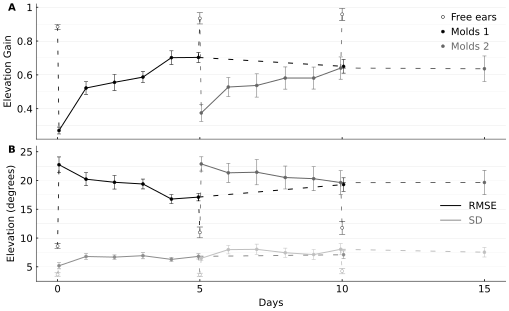
\includegraphics[width=18cm, center]{../Results/figures/fig5/fig5}
	\caption{Time course of vertical localization performance. White dots indicate performance with free ears, black and grey dots indicate performance with molds 1 and molds 2, respectively. Data points represent the mean across participants (ears free: n = 15, molds 1: n = 14, molds 2: n = 13). Error bars show the standard error. Slim dotted lines plot changes in localization performance after mold insertion and removal. Thick dotted lines show differences between the last test of the adaptation period and the final adaptation persistence test with each set of molds. \textbf{A}, Evolution of EG and \textbf{B}, localization error (RMSE) and response variability (SD) on the vertical plane throughout the two consecutive adaptation periods. Participants EG was reduced while RMSE and SD were increased after insertion of earmolds. EG and RMSE recovered within each of the two five-day adaptation periods, while SD further increased. Participants' EG recovered faster with the first set of molds than with the second set. After each mold removal, EG returned to baseline levels whereas RMSE increased compared to the first test with free ears (white dots on day 5 and 10). Although EG with molds 1 increased during adaptation to molds 2, adaptation persistence did not differ between the two sets of earmolds.}
        \label{fig:adaptation}
\end{figure}

 %% topic 4 adaptation(general adaptation, rate of adaptation m1/m2, generalisability, aftereffect, persistence)
 
\subsection{Participants adapted to two novel sets of DTFs}
 
Participants wore the two different sets of earmolds during two consecutive five-day adaptation periods. Adaptation was driven by multisensory experience while wearing the molds throughout the day, accompanied by five sessions of daily sensory-motor training at the lab. Vertical sound localization performance improved significantly for both sets of earmolds except for response variability (SD), which increased throughout the adaptation period (\cref{fig:adaptation}, one-tailed Wilcoxon signed rank tests of vertical localization on day 0 vs day 5 with earmolds; molds 1: EG: $p = 3 \times 10^{-5}$, RMSE: $p = 6 \times 10^{-5}$, SD: $p = 0.0042$; molds 2: EG: $p = 0.0002$, RMSE: $p = 0.032$, SD: p = 0.0081). As expected, horizontal localization was not affected by adaptation to the earmolds (one-tailed Wilcoxon signed rank tests of horizontal localization on day 0 vs day 5 with earmolds; molds 1; RMSE: $p = 0.555$, SD: $p = 0.467$, molds 2; RMSE: $p = 0.485$, SD: $p = 0.515$). %\subsection{Adaptation was generalizable}
To rule out the possibility of participants memorizing location-specific spectral features of the training stimuli in the localization test, the test was repeated with a subset of six participants on the last day of each adaptation period using stimuli of random spectral content (USOs). The effect of USO stimuli on vertical localization error did not differ between adapted earmolds and free ears indicating that generalizable perceptual learning had taken place (Friedman test; differences in vertical RMSE between pink noise and USO localization across conditions; Ears free: $-0.38 \pm 1.82$, Earmolds 1: $2.5 \pm 0.46$, Earmolds 2: $-0.15 \pm 0.45, p = 0.135$).

\subsection{No indication of metaplasticity in the adaptation to the second set of earmolds}

To investigate effects of metaplasticity, i.e., a faster relearning of sound localization with new pinna shapes after previously adapting to a different set of pinna modifikations, adaptation was compared between the first and the second set of molds. To quantify the rate of adaptation across participants and earmolds independent of initial acoustic disruption caused by the molds, the gain in localization performance during adaptation (performance on day 0 vs day 5) was divided by the initial performance drop on day 0. Individual rates of adaptation for each set of molds varied continuously and did not fall into discernable groups. Participants' adaptation rates in EG were higher with the first set of molds than with the second set. No differences between earmold adaptation rates were found for vertical RMSE (one-tailed Wilcoxon signed rank test of performance gain from day 0 to day 5 divided by initial performance drop; molds 1 vs molds 2; RMSE: 0.34 $\pm$ 0.06 vs 0.26 $\pm$ 0.09, $p = 0.2065$, EG: 0.7 $\pm$ 0.04 vs 0.45 $\pm$ 0.07, $p = 0.0122$). Individual adaptation rates with the first and second set of molds were positively related, although not significant (Spearman correlation coefficient: $r = 0.47, p = 0.142$). 

 % VSI dissimilarity and RMSE
 \begin{wrapfigure}[15]{l}{12.5cm}
\centering
    \raisebox{0pt}[\dimexpr\height+1.6\baselineskip\relax]{
        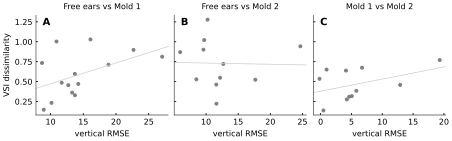
\includegraphics[width=12cm]{../Results/figures/fig6/fig6}}
	\caption{Acoustic dissimilarity and localization performance. Relation between VSI dissimilarity and vertical RMSE after mold insertion; \textbf{A}, with molds 1 compared to free ears, \textbf{B}, with molds 2 compared to free ears, \textbf{C}, with molds 2 compared to molds 1. Behavior with the second set of earmolds was better explained by acoustic dissimilarity to the previously adapted earmolds than to participants' native ears.}
	\label{fig:vsi_dis_rmse}
\end{wrapfigure}
\noindent%\vspace{-3\baselineskip}

\subsection{Effects of VSI dissimilarity on the disruption of localization performance across pinna shapes}

To test whether acoustic and behavioral effects of the earmolds were related, VSI dissimilarity between DTFs in the 5.7 – 13.5 kHz band with and without molds was compared to the decrease in participant’s localization performance after insertion of the earmolds. A trend of increasing vertical RMSE for larger acoustic differences was found for the first set of earmolds (\cref{fig:vsi_dis_rmse} A, Spearman correlation of VSI dissimilarity between free ears and molds 1 and increase in vertical RMSE after mold 1 insertion: $r = 0.43, p = 0.122$). No such trend was found for vertical localization and VSI dissimilarity between free ears and the second set of molds (\cref{fig:vsi_dis_rmse} B, Spearman correlation of vertical RMSE in the first test with molds 1 compared to free ears baseline and VSI dissimilarity: $r = - 0.18, p = 0.5926$). Because initial vertical localization accuracy with the second earmolds could depend on acoustic similarities to the previously learned set, differences in localization performance on the last day of adaptation to earmolds 1 and the initial test with the earmolds 2 were compared to the VSI dissimilarity between both sets of molds. A trend of increasing vertical error with greater acoustic dissimilarity between the first and second set of earmolds was found (\cref{fig:vsi_dis_rmse} C, Spearman correlation of increase in vertical RMSE from the last test with molds 1 to the first test with molds 2 and VSI dissimilarity between consecutive earmolds: $r = 0.35, p = 0.2847$). 

\subsection{Free ears localization accuracy decreased during adaptation}

Previous studies reported the absence of an aftereffect on localization performance with free ears after adaptation to new spectral cues for sound localization (\citet{hofman_relearning_1998}, \citet{trapeau_fast_2016}). To confirm these findings, free ears localization accuracy was measured immediately after earmolds were removed at the end of each adaptation period. No aftereffect was found for EG (SD?) but an increasing impact on participants’ vertical localization accuracy with their native ears was observed after each adaptation period (\cref{fig:adaptation} B, one-tailed Wilcoxon signed rank test, vertical RMSE; free ears baseline vs free ears day 5: $p = 0.002$, free ears baseline vs free ears day 10: $p = 0.0006$). 

\subsection{Vertical localization accuracy with the first earmolds decreased during adaptation to the second molds}

To investigate whether learning a new set of spectral cues for sound localization interfered with a previously learned set, earmolds were reinserted five days after mold removal and localization was re-measured. During the five days after the first earmolds were removed, participants adapted to another set of pinna modifications. The second set of earmolds served as a control because participants were not exposed to new spectral cues in the five days following mold 2 removal (see \cref{fig:adaptation}). Participants vertical localization accuracy with molds 1 was significantly decreased after five days of adaptation to the second molds (RMSE with molds 1 on day 5: 17.12 $\pm$ 0.65 and day 10: 19.3 $\pm$ 1.17, one-tailed Wilcoxon signed rank test, $p = 0.015$). Other metrics of localization performance did not differ significantly (one-tailed Wilcoxon signed rank test of performance with molds 1 on day 5 vs day 10; EG: $p = 0.1514$, SD: $p = 0.2997$). Localization performance with the second molds remained unchanged after 5 days with free ears (performance with molds 2 on day 10 vs day 15; RMSE: 19.64 $\pm$ 0.91 vs 19.66 $\pm$ 1.08, EG:  0.64 $\pm$ 0.03 vs 0.64 $\pm$ 0.06, SD:  8.05 $\pm$ 0.79 vs 7.54 $\pm$ 0.54). Adaptation persistence was defined as the difference between the last test with molds in the adaptation period and the final persistence tests with molds 1 and 2 on days 10 and 15, respectively. No difference in adaptation persistence was found between the first and second set of molds (one-tailed Wilcoxon signed rank test of adaptation persistence with molds 1 vs molds 2; RMSE: $p = 0.2119$, EG: $p = 0.2349$, SD: $p = 0.1902$). \cref{fig:response_evo} shows the evolution of response pattern with both sets of earmolds averaged across participants throughout the time course of the experiment.

% response evolution plot
 \begin{figure}[ht]
	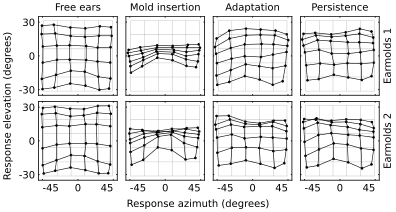
\includegraphics[width=14cm, center]{../Results/figures/fig7/fig7}
	\caption{Change of response pattern throughout the experiment. Grey panels show sound target locations, averaged for targets belonging to similar directions by dividing the target space into twenty-five half-overlapping sectors \citep{hofman_relearning_1998}. Black dots represent sound localization responses for each target averaged across all participants. The first and second row show behavioral impact, subsequent adaptation and adaptation persistence with molds 1 and 2, respectively.}
        \label{fig:response_evo}
\end{figure}

